\widowpenalty=10000
\clubpenalty=10000
\section{Objetivo del Informe}
Presentar los avances documentales y técnicos del proyecto Escanea y Entra,
incluyendo las pruebas preliminares de reconocimiento facial, para exponer
los resultados disponibles y las actividades pendientes.

\section{Alcance del Avance}
El proyecto estudia la posibilidad de integrar un sistema de control de
acceso en el TESCHA. La propuesta de investigación se centra en códigos QR
dinámicos y en su efecto sobre el tiempo de validación y la longitud de la
fila. Durante la exploración de alternativas se desarrolló una prueba de
concepto de reconocimiento facial y se registraron intentos de calibración
con comprobación de vida.

Este informe presenta la documentación del proyecto y la evidencia de banco
disponible al 13 de octubre de 2026. Los resultados faciales permiten
examinar el funcionamiento de esa prueba de concepto. La evaluación del
acceso del TESCHA requiere todavía documentar las mediciones de campo y los
resultados del prototipo basado en QR.

También se incorpora una sesión adicional con cámara en vivo, realizada el
mismo día a las 19:04, en la que se obtuvieron capturas de localización de
rostro y detección de parpadeo. Esta evidencia visual documenta el módulo de
pose del prototipo y se presenta por separado de los 45 intentos del CSV.

\section{Avances Documentados}
Se elaboraron el planteamiento del problema, la pregunta de investigación,
los objetivos y los instrumentos de diagnóstico. El planteamiento se
presenta en texto corrido, de lo general a lo particular, con la pregunta al
final. Los objetivos específicos siguen una secuencia desde el diagnóstico
hasta la evaluación del piloto. La importancia y la viabilidad se reúnen en
la justificación del documento completo.

En el componente técnico se dispone de programas para registrar sujetos,
reconocer rostros, aplicar comprobaciones de vida y guardar los resultados
de cada intento. El registro almacena vectores por motor. El código ofrece
las opciones SFace, buffalo\_s y buffalo\_l; el CSV analizado contiene
resultados únicamente de buffalo\_l. También existe un programa que guía
sesiones por condición y otro que resume los resultados.

\begin{table}[htbp]
\caption{Estado de los Avances y su Evidencia}
\label{tab:avances-estado}
{\small\linespread{1}\selectfont
\begin{tabular}{@{}P{3.7cm}P{4.4cm}P{4.8cm}@{}}
\toprule
Componente & Avance disponible & Evidencia \\
\midrule
Documento de investigación & Planteamiento, objetivos, justificación y
metodología redactados & Documento completo y versión de planteamiento y
objetivos. \\[0.5em]
Instrumentos de diagnóstico & Encuesta, entrevista y hoja de observación
elaboradas & Apéndices A, B y C del documento completo. \\[0.5em]
Prueba de concepto facial & Registro, reconocimiento y comprobación de vida
implementados en el código & Programas de registro, reconocimiento y vida;
vectores disponibles para el código s01. \\[0.5em]
Pruebas de calibración & 45 intentos guardados y resumidos por condición &
Archivo vigente de resultados del 13 de octubre de 2026. \\[0.5em]
Comparación con QR y NFC & Resultados por documentar en la evidencia
revisada & El CSV consultado contiene registros faciales. \\[0.5em]
Evaluación en el acceso & Resultados de campo por documentar & La evidencia
consultada corresponde a pruebas de banco. \\
\bottomrule
\end{tabular}}
\tablenote{Elaboración propia a partir de los archivos del proyecto y de la
copia de evidencias del reconocimiento facial. La existencia de un
instrumento o programa se distingue de su aplicación en el acceso.}
\end{table}

\section{Pruebas Preliminares de Reconocimiento Facial}
\subsection{Modalidades y Registro}
La implementación combina el reconocimiento del rostro con una comprobación
de vida. La modalidad pasiva
evalúa un cuadro sin solicitar movimientos. La activa solicita giros,
parpadeo y retorno al frente, y comprueba que la identidad se mantenga al
final. La modalidad ambas aplica primero la comprobación pasiva y continúa
con el reto activo cuando la decisión previa permite avanzar.

La base utilizada contiene 45 intentos del 13 de octubre de 2026, registrados
entre las 16:47:56 y las 17:29:09. Se distribuyen en 20 intentos de la modalidad
ambas, 20 de la pasiva y 5 de la activa. Todos están asociados al identificador
s01 y a condiciones de calibración. La etiqueta «otras personas» no permite
determinar cuántas personas distintas participaron en esos cinco intentos.

Se tomó como fuente el archivo vigente de resultados. El respaldo contiene
20 marcas de tiempo coincidentes con este archivo, por lo que se conservó
como antecedente sin sumarlo al total. En el informe se utilizan las
etiquetas de condición y resultado esperado del archivo vigente.

\subsection{Criterios de Lectura de los Resultados}
Un intento es correcto cuando se acepta al sujeto esperado o se rechaza una
entrada etiquetada para rechazo. Un falso rechazo ocurre cuando el rostro
que debía aceptarse es rechazado. Una falsa aceptación ocurre cuando se
acepta una entrada que debía rechazarse o se acepta con una identidad
distinta de la esperada.

El campo de tiempo registra el intervalo desde que se inicia el intento con
la tecla de captura hasta que se obtiene la decisión. En la modalidad activa
incluye la respuesta de la persona al reto. La implementación inicia este
cronómetro después de obtener el cuadro inicial de la cámara, de modo que
el dato no representa el tiempo completo de llegada, colocación y cruce de
un acceso.

\subsection{Decisiones Registradas}
En conjunto se registraron 43 decisiones correctas de 45 intentos: 18 de los
20 intentos etiquetados para aceptación fueron aceptados y los 25
etiquetados para rechazo fueron rechazados. La
Tabla~\ref{tab:avances-resultados} presenta el desglose que permite
interpretar cada modalidad y condición.

\begin{table}[htbp]
\caption{Decisiones Registradas en las Pruebas de Calibración}
\label{tab:avances-resultados}
{\small\linespread{1}\selectfont
\begin{tabular}{@{}P{1.7cm}P{3.4cm}rrrr@{}}
\toprule
Modo & Condición & Intentos & Aciertos & FR & FA \\
\midrule
Ambas & Rostro real & 5 & 5/5 & 0 & 0 \\[0.5em]
Ambas & Fotografía de s01 & 10 & 10/10 & 0 & 0 \\[0.5em]
Ambas & Otras personas & 5 & 5/5 & 0 & 0 \\[0.5em]
Pasiva & Rostro real & 10 & 9/10 & 1 & 0 \\[0.5em]
Pasiva & Foto en celular & 10 & 10/10 & 0 & 0 \\[0.5em]
Activa & Rostro real & 5 & 4/5 & 1 & 0 \\[0.5em]
\bottomrule
\end{tabular}}
\tablenote{Elaboración propia a partir del CSV vigente. Todos los registros usan el motor buffalo\_l. FR = falsos rechazos; FA = falsas aceptaciones. Un acierto corresponde a aceptar la identidad esperada o rechazar un intento etiquetado para rechazo. Los intentos son repeticiones de calibración.}
\end{table}


En la modalidad pasiva se aceptó el rostro real en 9 de 10 intentos; el
rechazo restante se registró con el detalle
\texttt{pasiva\_rostro\_cortado}. En la activa hubo 4 aceptaciones de
5 intentos con rostro real; el otro se rechazó por no completar el parpadeo.
En ambas se aceptaron los 5 intentos con rostro real y se rechazaron los
10 intentos de fotografía y los 5 etiquetados como otras personas.

La modalidad pasiva también rechazó los 10 intentos con una foto en celular.
Estos resultados describen las presentaciones incluidas en el archivo. Los
casos de fotografía del modo ambas se registran como fotografía de s01, sin
especificar el soporte utilizado.

\subsection{Tiempos de Decisión}
Los tiempos medios con rostro real fueron 216,4 milisegundos para la
modalidad pasiva, 5520,6 para la activa y 6008,9 para ambas. Las dos últimas
incluyen el tiempo de realización del reto. En la modalidad ambas, los casos
rechazados antes del reto activo registraron tiempos inferiores, por lo que
conviene interpretar cada condición por separado.

\begin{table}[htbp]
\caption{Tiempos de Decisión por Condición}
\label{tab:avances-tiempos}
{\small\linespread{1}\selectfont
\begin{tabular}{@{}P{1.5cm}P{3.1cm}rrr@{}}
\toprule
Modo & Condición & Media (ms) & Mediana (ms) & Máx. (ms) \\
\midrule
Ambas & Rostro real & 6008,9 & 6494,4 & 7044,4 \\[0.5em]
Ambas & Fotografía de s01 & 245,9 & 215,2 & 300,7 \\[0.5em]
Ambas & Otras personas & 234,2 & 215,4 & 301,0 \\[0.5em]
Pasiva & Rostro real & 216,4 & 221,8 & 275,5 \\[0.5em]
Pasiva & Foto en celular & 207,1 & 218,9 & 243,5 \\[0.5em]
Activa & Rostro real & 5520,6 & 5464,2 & 7231,5 \\[0.5em]
\bottomrule
\end{tabular}}
\tablenote{Elaboración propia. Se incluyen todos los intentos de cada condición, también los rechazados. En las modalidades activa y ambas, el tiempo incluye la realización del reto. En ambas, un rechazo previo puede detener el proceso sin ejecutar el reto activo.}
\end{table}


\clearpage
\begin{figure}[!ht]
\caption{Tiempo Medio de Decisión en los Intentos con Rostro Real}
\label{fig:avances-tiempos}
\centering
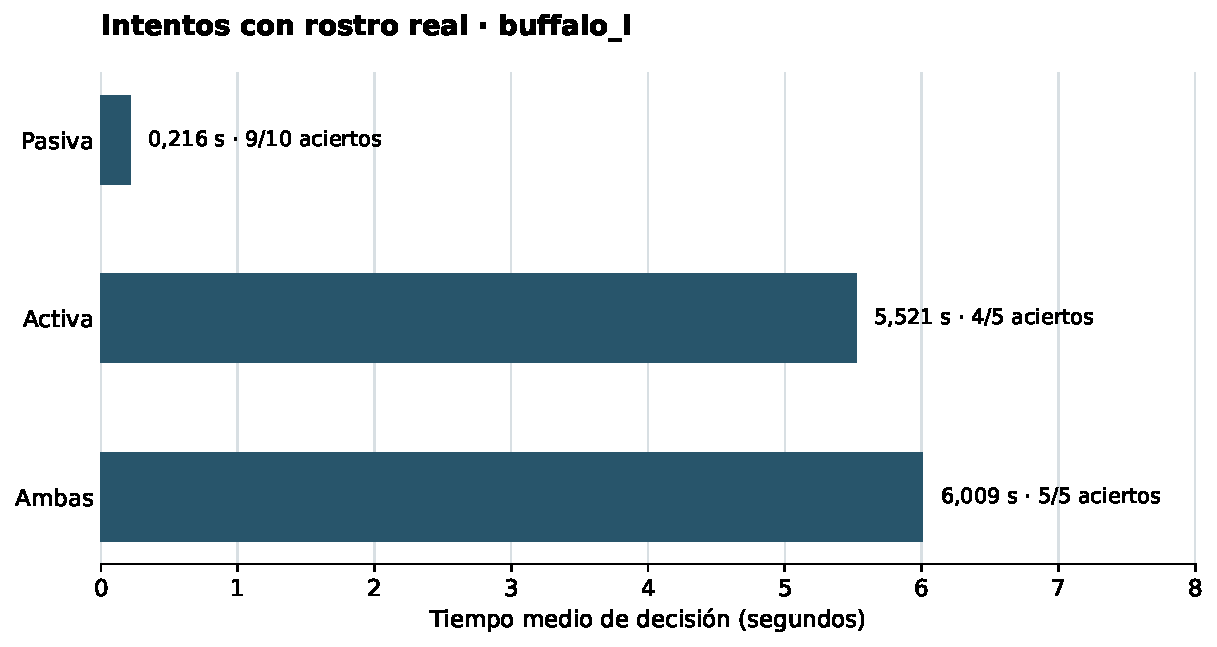
\includegraphics[width=0.96\linewidth]{evidencias/avances-2026-10-13/tiempos-rostro-real.pdf}
\figurenote{Elaboración propia con el CSV vigente. Las etiquetas indican
tiempo medio y aciertos por intentos. Se incluyen los rechazos en los
promedios. Activa y ambas incorporan la duración del reto; las condiciones
son de calibración y tienen distinto número de repeticiones.}
\end{figure}

\section{Interpretación del Avance}
La evidencia muestra que se dispone de un proceso que registra sujetos,
realiza reconocimiento y comprobación de vida y guarda decisiones y tiempos.
También permitió identificar dos situaciones para revisar: el encuadre del
rostro durante la comprobación pasiva y la ejecución del parpadeo en el reto
activo. Esos hallazgos orientan ajustes de uso y nuevas pruebas.

Los 45 intentos son repeticiones de calibración asociadas a un mismo código,
con grupos pequeños y desiguales. Los aciertos observados describen esta
sesión; todavía se requieren sesiones con más participantes y condiciones
registradas para estimar el desempeño en la población del TESCHA.

El archivo no conserva por intento el equipo de cómputo, la fuente de
cámara, las condiciones de iluminación ni la versión y configuración
exactas del programa. Las opciones descritas en este informe proceden del
código disponible al realizar la copia. Esta información deberá acompañar
las siguientes sesiones para facilitar su reproducción.

En los registros analizados no aparecen ensayos de QR, NFC, SFace,
buffalo\_s o reconocimiento sin comprobación de vida. Para comparar tiempos
entre tecnologías será necesario medir el mismo recorrido de validación.
La interpretación del efecto en la fila requiere además datos del acceso.

\section{Próximas Actividades}
\begin{itemize}
\interlinepenalty=10000
\item Registrar el equipo, la cámara, la configuración y las condiciones de
cada sesión antes de ampliar las pruebas.
\item Revisar el encuadre y las instrucciones del reto a partir de los dos
falsos rechazos observados.
\item Ampliar los participantes y completar las condiciones previstas de
iluminación y presentación de fotografías con identificación clara de cada caso.
\item Obtener pruebas comparables de QR y NFC con un criterio común de
inicio y fin de la validación.
\item Documentar la integración del prototipo de acceso y las mediciones de
campo necesarias para evaluar su efecto en el TESCHA.
\end{itemize}

\section{Evidencias del Informe}
La evidencia numérica procede de la carpeta de reconocimiento facial
proporcionada por el equipo. La copia conservada en
\path{evidencias/avances-2026-10-13/} contiene el CSV vigente, su respaldo,
la documentación, los programas y el resumen utilizado para las tablas y la
gráfica. El registro de procedencia identifica los archivos empleados.

Las capturas reales de la sesión adicional se conservan en la subcarpeta
\path{camara/}. Su registro incluye la fecha, el evento detectado y las
dimensiones de cada cuadro. Esta sesión utiliza el módulo de pose del
prototipo y documenta la localización del rostro y el parpadeo.

\clearpage
\section{Evidencia Visual de las Pruebas}
Las siguientes imágenes se obtuvieron de la cámara durante una sesión con
un participante voluntario. La primera documenta la localización del rostro
y la segunda el parpadeo detectado por el módulo de pose.

\begin{figure}[!ht]
\caption{Captura de la Prueba de Localización del Rostro}
\label{fig:avances-camara-deteccion}
\centering
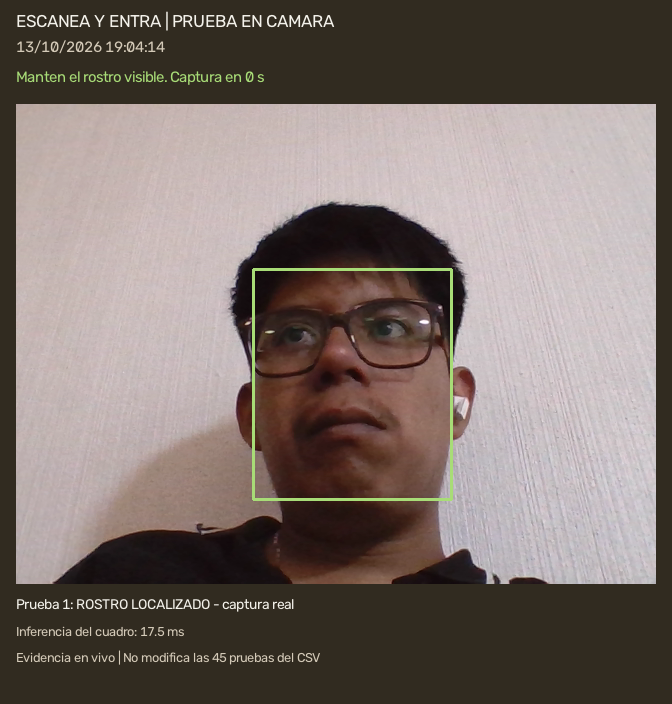
\includegraphics[width=0.85\linewidth]{evidencias/avances-2026-10-13/camara/01-deteccion.png}
\figurenote{Captura real del 13 de octubre de 2026 a las 19:04:14. El recuadro
indica el rostro localizado. El tiempo mostrado corresponde al procesamiento
de ese cuadro.}
\end{figure}

\clearpage
\begin{figure}[!ht]
\caption{Captura de la Prueba de Detección de Parpadeo}
\label{fig:avances-camara-parpadeo}
\centering
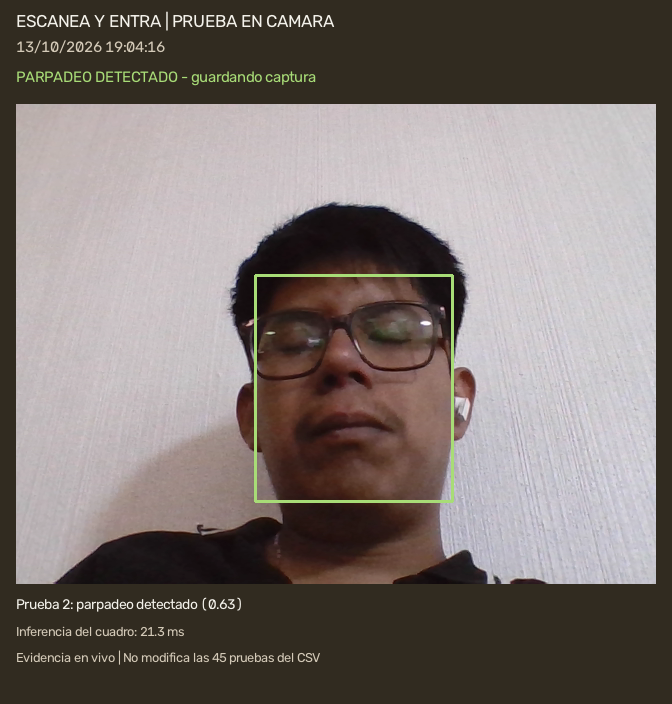
\includegraphics[width=0.85\linewidth]{evidencias/avances-2026-10-13/camara/02-parpadeo.png}
\figurenote{Captura real del 13 de octubre de 2026 a las 19:04:16. El módulo
registró una puntuación de parpadeo de 0,63, superior al umbral de 0,50
utilizado en esta prueba. La sesión adicional documenta detección y movimiento;
el resumen estadístico corresponde a los 45 intentos del archivo original.}
\end{figure}
